\chapter{Preliminaries}
\label{chapter:preliminaries}

The following Sections describe all the concepts required for the reader to understand the proposed method in this thesis. However, it is still assumed that the reader has some basic knowledge about programming and computational intelligence. For this reason, the following concepts are focused on terms related to finance, specifically to trading and financial markets, and to agent-based models and multi-agent systems.

\section{Financial Market}
\label{section:financial-market}

A financial market represents

\section{Trading Strategy}
\label{section:trading-strategy}

A trading strategy is a set of processes that help a trader to determine different aspects of a financial market and to later make trading decisions based on these aspects. For example, a trader can determine that a market is going to follow an uptrend -- that is, that the price of a financial market is going to rise -- and take the decision of buying shares of the asset of that financial market. Trading strategies can vary in complexity: some can use simple moving averages to determine trends and entry points, and others can take into consideration many different indicators, as well as the trader's experience.

An untrained person can think that trading a financial market only involves deciding when to buy or sell a market. Nevertheless, the possible decisions can be as complex as the strategy used to determine them. For instance, when traders are about to open a new buy or sell order, they also need to decide the size of the order, or how many units are going to be bought or sold. These units can be shares in a stock market or an amount of a currency in foreign exchange markets, for example. This order can also be delayed: the trader can decide that an order will be opened when a certain amount of time passes or when certain price in a financial market is reached. Additionally, the trader can specify \textit{stop loss} and/or \text{take profit} prices: after executing a buy or sell order, if the market reaches certain price, the trade has to be cancelled, stopping any losses or taking any profits that that trade generated since it was created.

The initial process of creating a trade order is complex, as noted in the previous paragraph, but decisions can also take place after a number of trade orders have been executed. The most obvious decision is when one should stop a trade. This particular decision has spawned several psychological research works, where the decision process is analyzed. A clear example is depicted in Figure \ref{figure:trading-psychology}, where the emotions that traders generally feel when experiencing a the earnings or losses of a trade are shown.

%% Amaury: I will create my own version of this chart (re-make it to match style)
%% Amaury: I will also cite this
\begin{figure}
\caption{Trading psychology}
\centering
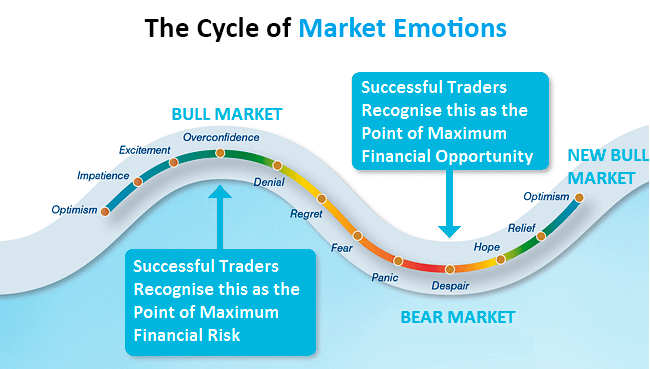
\includegraphics[width=1.0\textwidth]{img/trading-psychology.png}
\label{figure:trading-psychology}
\end{figure}

Stopping a trade does not only involve emotions, as a thorough analysis of the market, about the current's account financial situation and the trades themselves needs to be performed. Regarding about the first step -- an analysis of the market -- it is worth mentioning that these analyses are usually different than those performed when deciding when to start trading a market. For example, in a stagnated market one could decide not to trade a market, but this does not necessarily mean that one should close trade orders in this situation; one could consider that this is a moment where trades need to be held until further price movements take place. A trader can also decide to \textit{partially} stop a trade; that is, a trader can decide to sell a certain amount of units from a trade, for example. Likewise, a trader can decide to acquire more units from the asset.

It is usual that a trader \textit{diversifies} its trading portfolio. Diversifying means that a trader starts trading a number of financial markets instead of focusing on a single market. The advantages of this %% Amaury: \cite
are that the risk diminishes, as the profits of trading some markets can compensate the losses obtained from trading other markets. Diversification can then make trading strategies even more complex, as a trader now needs to take into consideration different markets. Additionally, markets usually affect the price movements of other markets, for example, if wheat price goes up, this can directly impact the price of McDonald's stock prices, as many of their products contain wheat-based ingredients. Furthermore, if McDonald's stock market is severely affected, this could negatively impact the United States' economy, as McDonald's is one of the most profitable companies in this country. Depending on the robustness of a trading strategy, all of these aspects can be considered to take a decision.

Trading strategies have existed since the activity of trading was created. To illustrate this, one can consider how the Japanese traded certain commodity markets, such as the rice market, using strategies based on candlestick patterns. %% Amaury: \cite
The Japanese charted the prices by representing the open, highest, lowest and close prices for a period of time using a figures that resemble candles and their wicks, as the ones seen in Figure \ref{figure:candlestick-chart}. The body of a candle in this type of charts represents the opening and the closing prices of a session, while the wick represents the lowest and highest prices that occured during the session.


%% These two will be redesigned to match the thesis document style
\begin{figure}
\caption{Example of a candlestick chart}
\centering
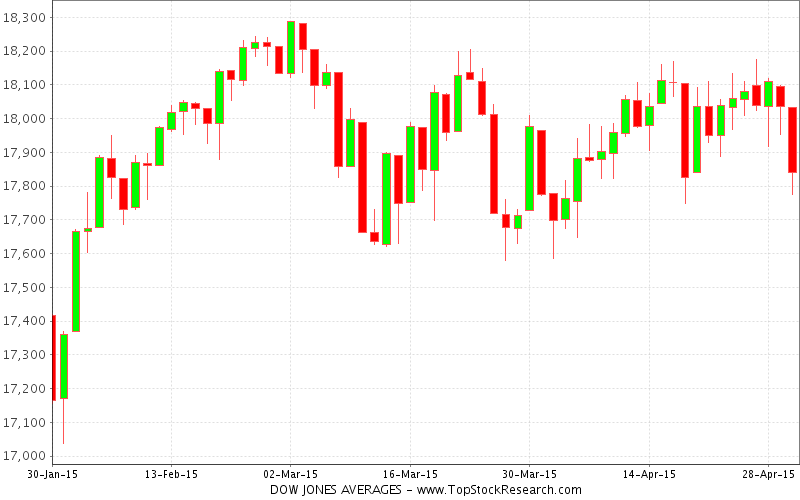
\includegraphics[width=1.0\textwidth]{img/candlestick-chart.png}
\label{figure:candlestick-chart}
\end{figure}

As mentioned before, Japanese traders noticed patterns that emerged in the candlestick charts. These patterns helped the traders to understand the current situation of a financial market and to take decisions based on these assumptions. Some example patterns are shown in Figure \ref{figure:candlestick-patterns}. For example, if a "bullish engulfing" or a "rising sun" candlestick pattern appears in the chart of a market, this is considered as a sign of a following uptrend -- which means that prices will increase. In contrast, if a "bearish engulfing" or "dark cloud cover" candlestick pattern appears, this signs a following downtrend -- which means that prices will decrease. Additionally, there are patterns that indicate that a market will start stagnating, such as the "harami" candlestick pattern. It is worth noting that these candlestick patterns are still used in modern trading strategies.

All the processes described above can be performed manually, i.e. a trader can look at price charts and start identifying candlestick patterns, draw moving averages over the chart, decide on the number of units to buy or sell, decide on take profit and stop loss levels, etc. However, with the introduction of computers to the financial world in the mid 20th century, automated or algorithmic trading was also introduced. % Amaury: \cite
Algorithmic trading help traders to partially or totally delegate trading tasks to computer software, where buy or sell transactions occur when a set of conditions are met. In this thesis, an automated trading strategy is part of the proposed method.

\begin{figure}
\caption{Example of candlestick patterns}
\centering
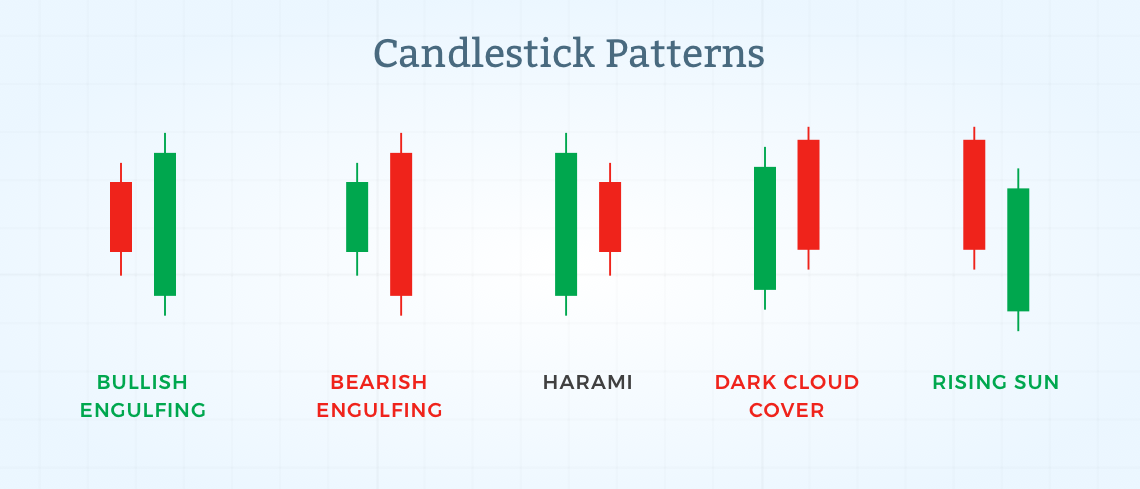
\includegraphics[width=1.0\textwidth]{img/candlestick-patterns.png}
\label{figure:candlestick-patterns}
\end{figure}

\section{Computational Intelligence}
\label{section:computational-intelligence}

\subsection{Fuzzy Sets}
\label{subsection:fuzzy-sets}

\subsection{Fuzzy Systems}
\label{subsection:fuzzy-systems}

\subsection{Fuzzy Systems Software}
\label{subsection:fuzzy-systems-software}

\subsection{Intuitionistic Fuzzy Sets}
\label{subsection:intuitionistic-fuzzy-sets}

\subsection{Intuitionistic Fuzzy Systems}
\label{subsection:intuitionistic-fuzzy-systems}

\subsection{Membership Function Design}
\label{subsection:membership-function-design}

\subsection{Genetic Programming}
\label{subsection:genetic-programming}

\section{Multi-agent Systems and Models}
\label{section:multi-agent-systems-and-models}

\section{Technical Analysis}
\label{section:technical-analysis}

\section{Retracements in Financial Markets}
\label{section:retracements-in-financial-markets}

